% Template for PLoS
% Version 3.5 March 2018
%
% % % % % % % % % % % % % % % % % % % % % %
\documentclass[10pt,letterpaper]{article}
\usepackage[top=0.85in,left=2.75in,footskip=0.75in]{geometry}
% FIGURES
\usepackage{graphicx}
\usepackage{pgf}
% amsmath and amssymb packages, useful for mathematical formulas and symbols
\usepackage{amsmath,amssymb}
% Use adjustwidth environment to exceed column width (see example table in text)
\usepackage{changepage}
% Use Unicode characters when possible
\usepackage[utf8x]{inputenc}
% textcomp package and marvosym package for additional characters
\usepackage{textcomp,marvosym}
% cite package, to clean up citations in the main text. Do not remove.
\usepackage{cite}
% Use nameref to cite supporting information files (see Supporting Information section for more info)
\usepackage{nameref,hyperref}
% line numbers
\usepackage[right]{lineno}
% ligatures disabled
\usepackage{microtype}
\DisableLigatures[f]{encoding = *, family = * }
% color can be used to apply background shading to table cells only
\usepackage[]{xcolor}
% array package and thick rules for tables
\usepackage{array}
% create "+" rule type for thick vertical lines
\newcolumntype{+}{!{\vrule width 2pt}}
% create \thickcline for thick horizontal lines of variable length
\newlength\savedwidth
\newcommand\thickcline[1]{%
  \noalign{\global\savedwidth\arrayrulewidth\global\arrayrulewidth 2pt}%
  \cline{#1}%
  \noalign{\vskip\arrayrulewidth}%
  \noalign{\global\arrayrulewidth\savedwidth}%
}
% \thickhline command for thick horizontal lines that span the table
\newcommand\thickhline{\noalign{\global\savedwidth\arrayrulewidth\global\arrayrulewidth 2pt}%
\hline
\noalign{\global\arrayrulewidth\savedwidth}}
% Text layout
\raggedright
\setlength{\parindent}{0.5cm}
\textwidth 5.25in 
\textheight 8.75in
% Bold the 'Figure #' in the caption and separate it from the title/caption with a period
% Captions will be left justified
\usepackage[aboveskip=1pt,labelfont=bf,labelsep=period,justification=raggedright,singlelinecheck=off]{caption}
\renewcommand{\figurename}{Fig}
% Remove brackets from numbering in List of References
\makeatletter
\renewcommand{\@biblabel}[1]{\quad#1.}
\makeatother
% Header and Footer with logo
\usepackage{lastpage,fancyhdr,graphicx}
\usepackage{epstopdf}
\pagestyle{fancy}
\fancyhf{}
\rfoot{\thepage/\pageref{LastPage}}
\renewcommand{\headrulewidth}{0pt}
\renewcommand{\footrule}{\hrule height 2pt \vspace{2mm}}
\fancyheadoffset[L]{2.25in}
\fancyfootoffset[L]{2.25in}
\lfoot{\today}
%% Include all macros below
\newcommand{\lorem}{{\bf LOREM}}
\newcommand{\ipsum}{{\bf IPSUM}}
%% END MACROS SECTION
%%%%%%%%%%%%%%%%%%%%%%%%%%%%%%%%%%%%%%%%%%%%%%%%%%%%%%%%%%%%%%%%%%%%%%%%%%%%%%%%%%%%%%%%%%


\begin{document}
\vspace*{0.2in}

% TITLE
\begin{flushleft}
{\Large
\textbf\newline{
Analysis of heatwaves in UKCP18 climate projections
}}
\newline
\\
Kevin Donkers\textsuperscript{1,2*}
\\
\bigskip
\textbf{1} Environmental Intelligence CDT, University of Exeter, Exeter, Devon, UK
\\
\textbf{2} Informatics Lab, Met Office, Exeter, Devon, UK
\\
\bigskip
* kevin.donkers@informaticslab.co.uk
\end{flushleft}


% ABSTRACT (below 300 words)
\section*{Abstract}
CLIMAR! Mention Climar framework!
As global average temperatures continue to increase under climate change, extreme events will become commonplace and previously impossible events the new extremes. The impacts of high temperatures  are far reaching and the increased likelihood of extreme heatwaves is already being felt, for instance with the 2003(??) European heatwave which caused **** excess deaths [cit]. In the UK the Met Office define a heatwave as three or more consecutive days of daily maximum temperatures exceeding a given threshold temperature, as defined by the local climatology[cit]. We use this to analyse the number and duration of heatwaves projected to occur in London under the UKCP18 climate projections. In addition we conduct this heatwave analysis using a Universal Thermal Climate Index (UTCI) adjustment to the maximum daily air temperature, which factors in humidity and windspeed to provide a more physiologically accurate representation of high temperatures. This could be used to overcome some of the assumptions posed in the Met Office heatwave definition in order to define a more universal heatwave definition.

% INTRODUCTION
\section*{Introduction}

Background:
- CLIMAR/Risk framework...

- Climate change global temperature increase
- European heatwave 2003 [cit Stott2004] = hottest european summer for 500 years
- European heatwave 2019 [cit Voutard2020] = record breaking
- UK heatwave mortality [cit johnson2005] and morbidity [cit smith2016]
- infrastructure impacts [cit Dawson et al., 2017]

As global mean temperatures increase due to climate change, heatwaves are expected to get hotter, longer and more frequent. 
Indeed we are already seeing many more unprecedented heatwaves in Europe, starting in 2003 with the hottest heatwave for 500 years \cite{Stott2004} and continuing to break records in 2019, the latter being statistically attributed to anthropogenic climate change. \cite{Vautard2020} 
The UK heatwave in August 2020 was another record breaker. \cite{Askew2020}
Heatwaves in the UK have been shown to increase human morbidity \cite{Smith2016}, mortality \cite{Johnson2004} and disruption to critical infrastructure. \cite{Dawson2016}






- WMO heatwave definition [cit WMO2018]
    - "A period of marked unusual hot weather
over a region persisting for at least three consecutive days during the warm period of the year based on local climatological con- ditions, with thermal conditions recorded above given thresholds." 

- Met Office heatwave definition [\cite{McCarthy2019}]
    - Important to challenge assumptions since dominant weather patterns may change in future 
    - "Despite the widespread usage, ... there is no unified definition, either within the United Kingdom or internationally." [\cite{McCarthy2019}]
    
    - 90th percentile of maximum daily temperature for July in years 1981-2010 within a county, rounded to nearest whole degree °C.

    - Critique of this method
        - Definition relies on climatology, but years in which climate change have already adjusted climatology were used. It is not clear for which years this shifting baseline is relevant.
        - Climatology includes some of the ten warmest years on record (since 2002)
        - Climatology includes 
        - Climatology arbitrarily defined on a county basis, despite marked variation within some county boundaries.
        - Definition has been made to balance responsibilities of national meteorological service messaging, in which public perception and frequency of messaging are key consideration.
        - However this is not so useful when applied to climate projection data decades in the future.
        - Physiologically significant physical parameters like humidity and wind speed not included 
    
- UTCI background
    - 

- Therefore a comparison of Met Office heatwave thresholds with UTCI heat stress thresholds is conducted in this paper.

\section*{Materials and methods}

\subsection*{UKCP18 Data}

- RCP8.5 climate forcing scenario
- Land Convection Permitting model
    - HadREM3-RA11M
    - driven by perturbed variants of the Met Office Unified Model Global Atmosphere GA7 model (HadREM3-GA705) at 12km resolution
    - The HadREM3-GA705 models were driven by perturbed variants of the global HadGEM3-GC3.05
- set of 12 model runs (ensemble members)
- 2.2km spatial resolution
    - Spatial average of Greater London area
    - Presumable mean
- Maximum daily air temperature at 1.5m altitude
- Supplemented with:
    - Daily mean relative humidity
    - Daily mean surface wind speed



\subsection*{Met Office heatwave analysis}


\subsection*{UTCI calculation}










% Results and Discussion can be combined.
\section*{Results}



Plots
- Decadal box plots
- Poisson fits
- Report poisson lambdas

Results:
- Compare tasmax, utci and utci10
- 

\section*{Discussion}

Implications:
- UTCI with met office threshold not good
- UTCI does pick out heatwaves, but less than plain air temperature

Ways to improve:
- Tmrt excluded from UTCI calculation because not enough data to calculate it
    - Assumed Ta=Tmrt, but this is a substantial assumption i.e. air in thermal equilibrium with surroundings
    - Will exclude urban heat island effects, which are substantial [cit]
    - To what extent is urban heat island already accounted for in UKCP air temperature data?
    - Tmrt can't be applied to UTCI retroactively (e.g. once Exposure has been calculated) since UTCI relies on a 6th order polynomial calculation including every iteration of using Tmrt
- Humidity and windspeed used in UTCI calculation are daily means so not at same time of day as tasmax
    - However they don't affect the temperature strongly, so source of error is minimal
    - Tmrt is source of bigger error since effect is larger
    - Covariance matrices?


Future exploration:
- Explore change in higher tiers of heat stress from UTCI data
- Tasmin (nighttime) temperatures ("tropical nights")
- Use incident radiation and cloud cover to improve UTCI calculation
- Use urban data to better model mean radiant temperature
- Use zero-inflated Poisson to fit heatwave duration graphs


\section*{Conclusion}




\cite{Askew2020}






\pagebreak

\bibliographystyle{plos2015}

\bibliography{CLIMAR-2021_Mar_report.bib}






% %%%%%%%%%%%%%%%%%%%%%%%%%%%%%%%%%%%%%%%%%%%%%%%%%%%%%%%%%%%%%%%%%%%%%%%%%%%%%%%%%%%%%%%%%%
% %%%%%%%%%%%%%%%%%%%%%%%%%%%%%%%%%%%%%%%%%%%%%%%%%%%%%%%%%%%%%%%%%%%%%%%%%%%%%%%%%%%%%%%%%%
% %%%%%%%%%%%%%%%%%%%%%%%%%%%%%%%%%%%%%%%%%%%%%%%%%%%%%%%%%%%%%%%%%%%%%%%%%%%%%%%%%%%%%%%%%%
% %%%%%%%%%%%%%%%%%%%%%%%%%%%%%%%%%%%%%%%%%%%%%%%%%%%%%%%%%%%%%%%%%%%%%%%%%%%%%%%%%%%%%%%%%%
% %%%%%%%%%%%%%%%%%%%%%%%%%%%%%%%%%%%%%%%%%%%%%%%%%%%%%%%%%%%%%%%%%%%%%%%%%%%%%%%%%%%%%%%%%%
\pagebreak
\section*{Supporting information}
% Include only the SI item label in the paragraph heading. Use the \nameref{label} command to cite SI items in the text.
\paragraph*{S1 Fig.}
\label{S1_Fig}
{\bf Bold the title sentence.} Add descriptive text after the title of the item (optional).



\subsection*{Subsection - Other sturff}



CO\textsubscript{2}


Eq~\ref{eq:schemeP}


Fig~\ref{fig1}


Table~\ref{table1} 


Citation~\cite{LaGennusa2005}




% Use "Eq" instead of "Equation" for equation citations.
\begin{eqnarray}
\label{eq:schemeP}
	\mathrm{P_Y} = \underbrace{H(Y_n) - H(Y_n|\mathbf{V}^{Y}_{n})}_{S_Y} + \underbrace{H(Y_n|\mathbf{V}^{Y}_{n})- H(Y_n|\mathbf{V}^{X,Y}_{n})}_{T_{X\rightarrow Y}},
\end{eqnarray}


% For figure citations, please use "Fig" instead of "Figure".
% Place figure captions after the first paragraph in which they are cited.
\begin{figure}[!h]
\caption{{\bf Bold the figure title.}
Figure caption text here, please use this space for the figure panel descriptions instead of using subfigure commands. A: Lorem ipsum dolor sit amet. B: Consectetur adipiscing elit.}
\label{fig1}
\end{figure}



\begin{itemize}
	\item First bulleted item.
	\item Second bulleted item.
	\item Third bulleted item.
\end{itemize}

% Place tables after the first paragraph in which they are cited.
\begin{table}[!ht]
\begin{adjustwidth}{-2.25in}{0in} % Comment out/remove adjustwidth environment if table fits in text column.
\centering
\caption{
{\bf Table caption Nulla mi mi, venenatis sed ipsum varius, volutpat euismod diam.}}
\begin{tabular}{|l+l|l|l|l|l|l|l|}
\hline
\multicolumn{4}{|l|}{\bf Heading1} & \multicolumn{4}{|l|}{\bf Heading2}\\ \thickhline
$cell1 row1$ & cell2 row 1 & cell3 row 1 & cell4 row 1 & cell5 row 1 & cell6 row 1 & cell7 row 1 & cell8 row 1\\ \hline
$cell1 row2$ & cell2 row 2 & cell3 row 2 & cell4 row 2 & cell5 row 2 & cell6 row 2 & cell7 row 2 & cell8 row 2\\ \hline
$cell1 row3$ & cell2 row 3 & cell3 row 3 & cell4 row 3 & cell5 row 3 & cell6 row 3 & cell7 row 3 & cell8 row 3\\ \hline
\end{tabular}
\begin{flushleft} Table notes Phasellus venenatis, tortor nec vestibulum mattis, massa tortor interdum felis, nec pellentesque metus tortor nec nisl. Ut ornare mauris tellus, vel dapibus arcu suscipit sed.
\end{flushleft}
\label{table1}
\end{adjustwidth}
\end{table}





\pagebreak


\begin{figure}
\begin{adjustwidth}{-2.25in}{0in}
    \begin{center}
        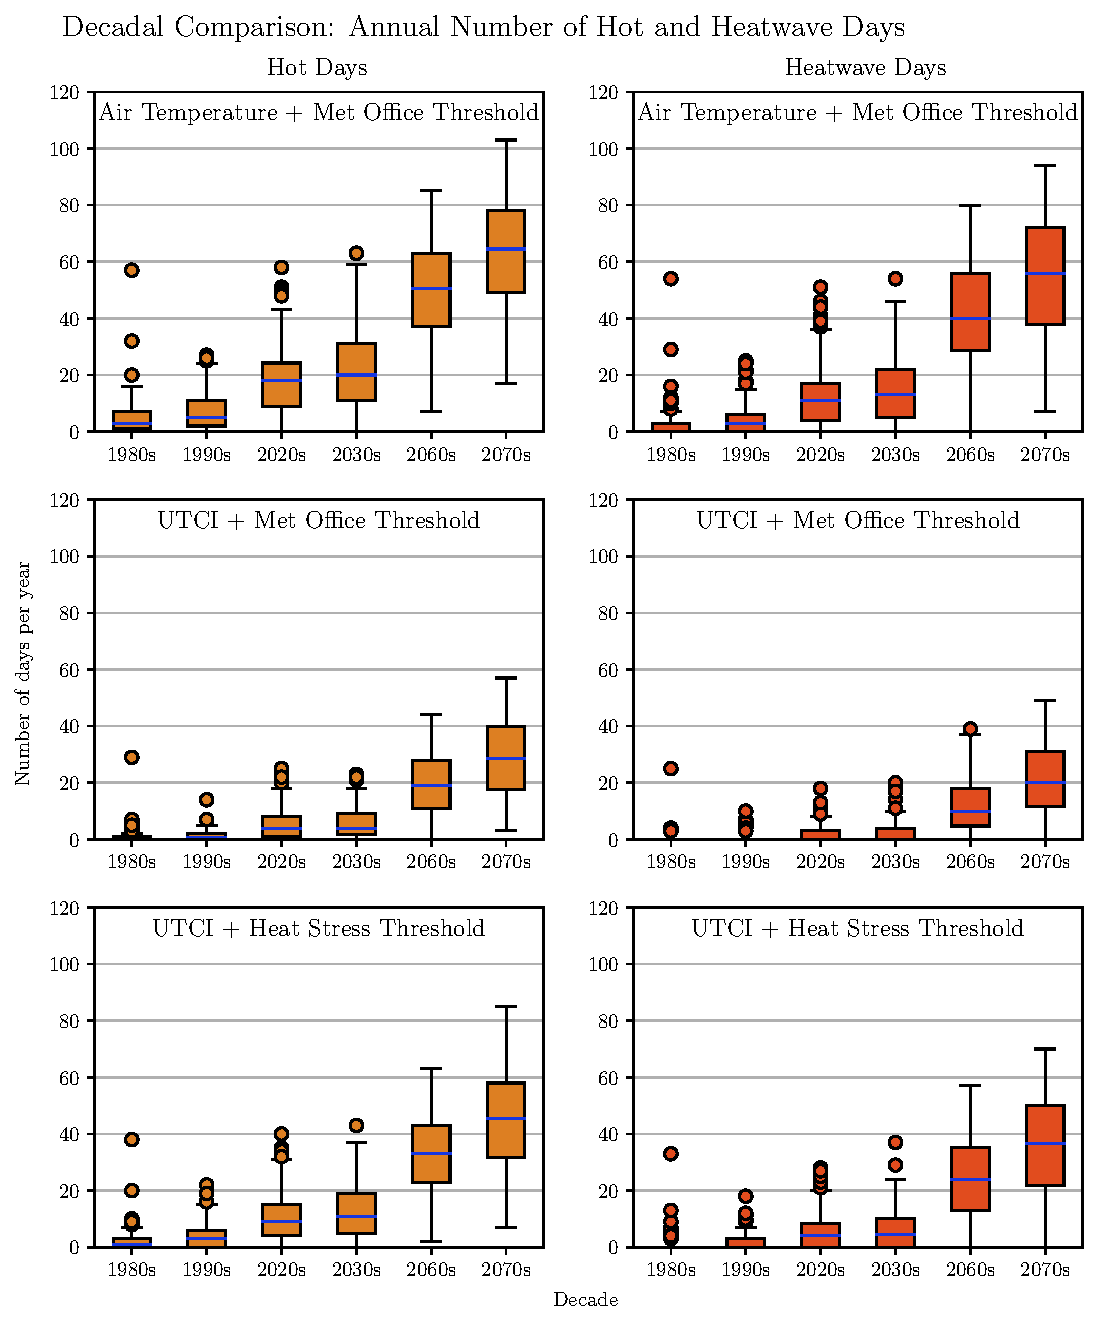
\includegraphics[width=0.9\linewidth]{./boxplots.pdf}
    \end{center}
    \caption{
    {\bf Annual number of hot and heatwave days increases over the decades modelled.}
    An accelerated increase is observed in the later decades of the 21\textsuperscript{st} century.
    Here hot days are defined as the total number of days in the year that exceed a threshold, whereas heatwave days are the total number of days in the year that are part of a continuous 3+ day heatwave. This analysis was done with raw and UTCI adjusted maximum daily air temperatures using thresholds defined by the Met Office and UTCI heat stress theory. Air temperature values for Greater London area used.
    }
    \label{boxplots}
\end{adjustwidth}
\end{figure}

\begin{figure}
\begin{adjustwidth}{-2.25in}{0in}
    \begin{center}
        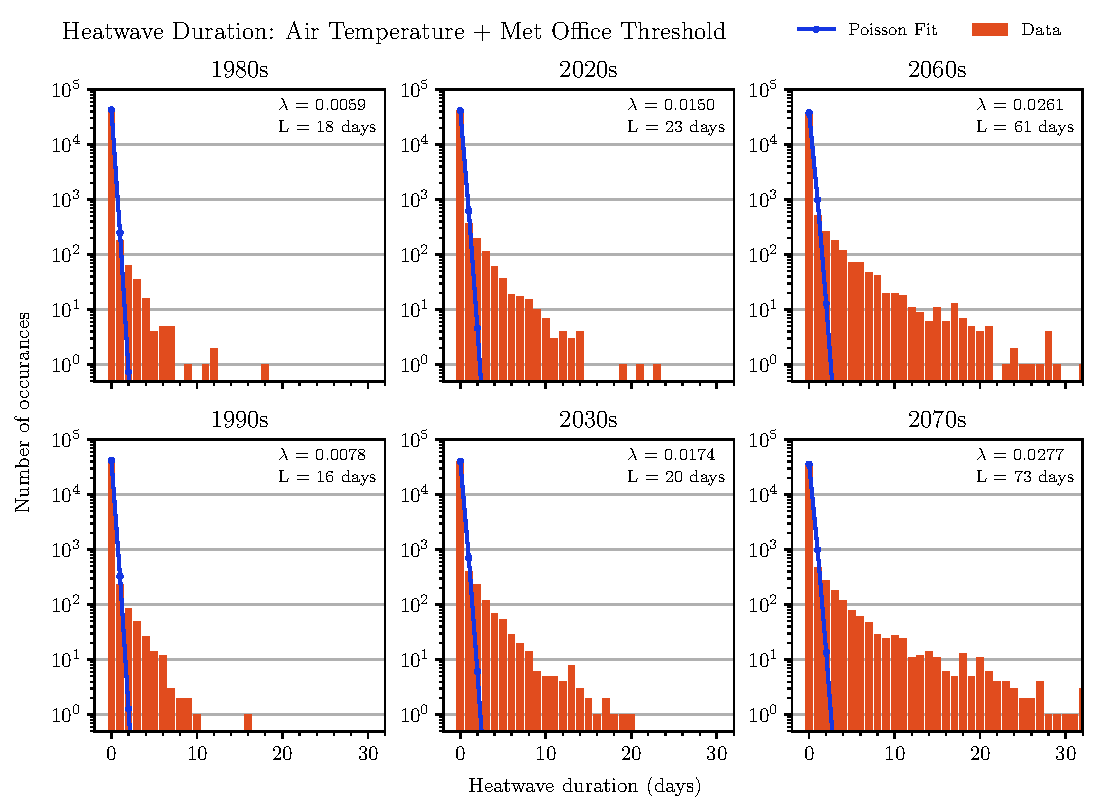
\includegraphics[width=\linewidth]{./tas_poisson.pdf}
    \end{center}
    \caption{
    {\bf Met Office heatwave definition predicts heatwaves up to 73 days long in the 2070s.}
    Comparison of all heatwave events across all years and ensemble members, grouped by decade.
    Here heatwave event duration is defined as a number of consecutive days in which the maximum daily air temperature exceeds the local climatologically defined threshold.
    Each decade has had a Poisson distribution fitted to it, with the resulting rate presented as $\lambda$.
    The longest contiguous heatwave in each decade is presented as $L$.
    Occurrence frequency is shown on a logarithmic scale so as to highlight low likelihood, high duration heatwave events.
    }
    \label{tas-poisson}
\end{adjustwidth}
\end{figure}

\begin{figure}
\begin{adjustwidth}{-2.25in}{0in}
    \begin{center}
        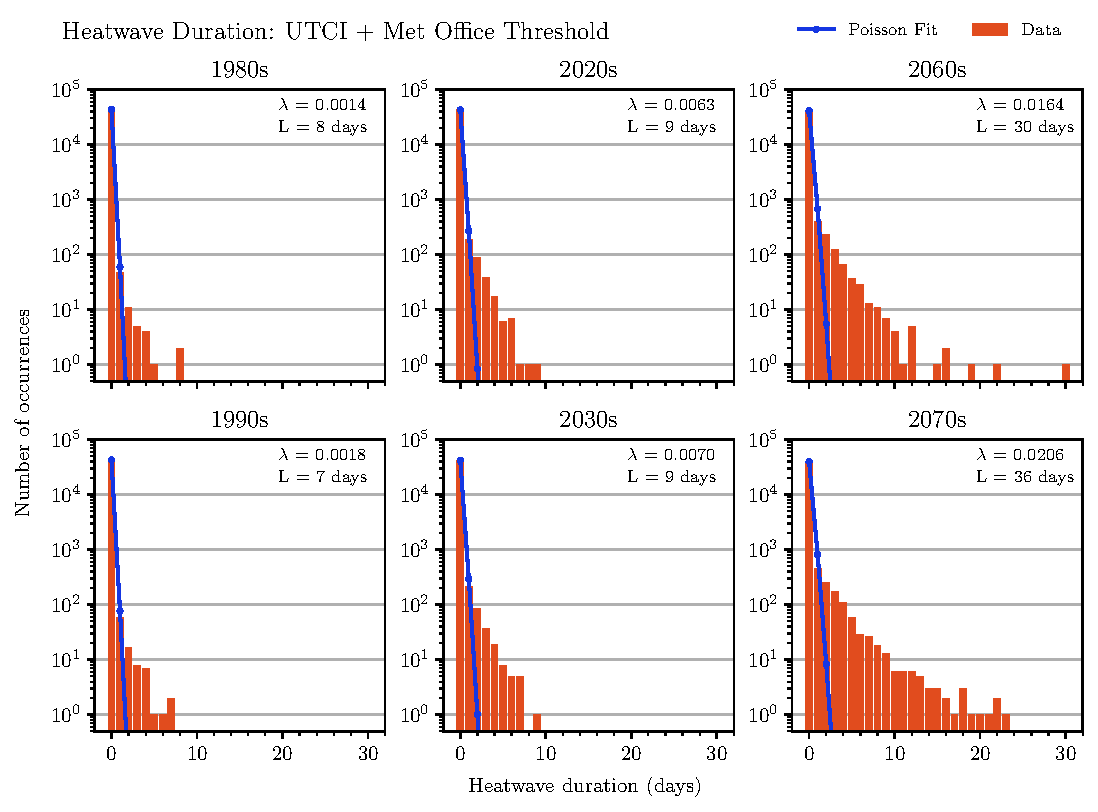
\includegraphics[width=\linewidth]{./utci_poisson.pdf}
    \end{center}
    \caption{
    {\bf UTCI with Met Office heatwave threshold predicts heatwaves up to 36 days long in the 2070s.}
    Comparison of all heatwave events across all years and ensemble members, grouped by decade.
    Here heatwave event duration is defined as a number of consecutive days in which the UTCI adjusted maximum daily air temperature exceeds the local climatologically defined threshold.
    Each decade has had a Poisson distribution fitted to it, with the resulting rate presented as $\lambda$.
    The longest contiguous heatwave in each decade is presented as $L$.
    Occurrence frequency is shown on a logarithmic scale so as to highlight low likelihood, high duration heatwave events.
    }
    \label{utci-poisson}
\end{adjustwidth}
\end{figure}

\begin{figure}
\begin{adjustwidth}{-2.25in}{0in}
    \begin{center}
        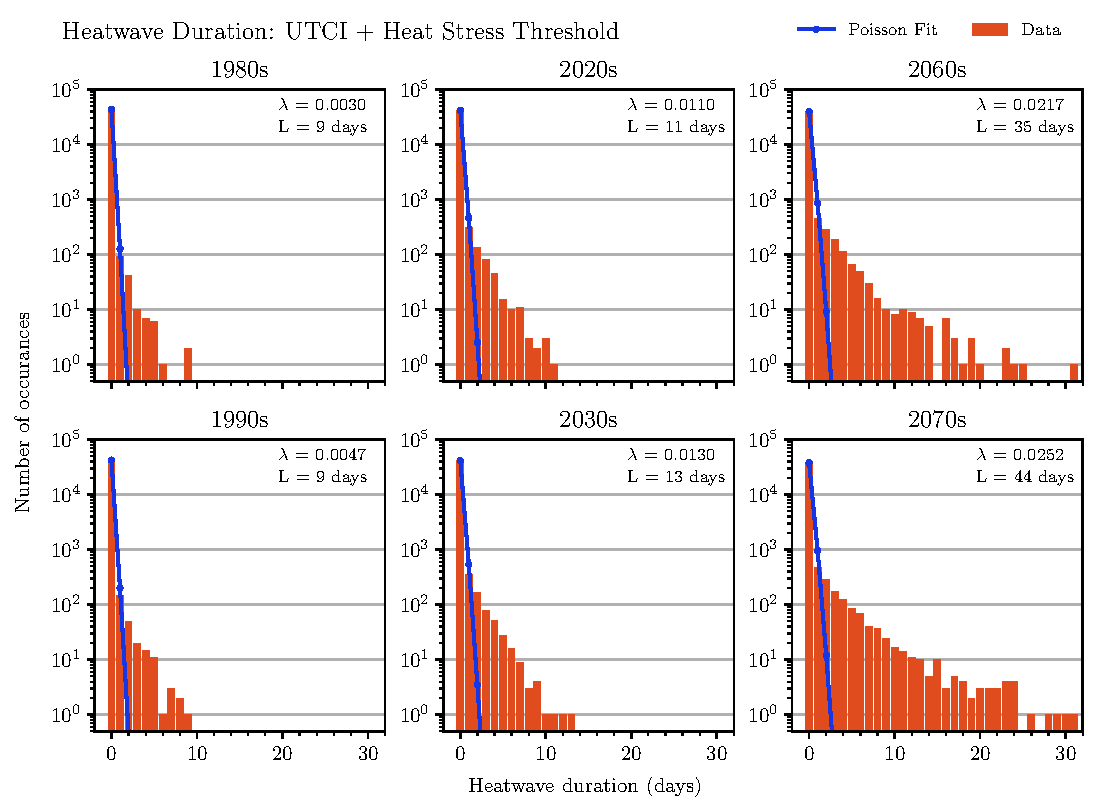
\includegraphics[width=\linewidth]{./u10_poisson.pdf}
    \end{center}
    \caption{
    {\bf UTCI heat stress definition predicts heatwaves up to 44 days long in the 2070s.}
    Comparison of all heatwave events across all years and ensemble members, grouped by decade.
    Here heatwave event duration is defined as a number of consecutive days in which the UTCI adjusted maximum daily air temperature exceeds the UTCI theoretical heat stress threshold.
    Each decade has had a Poisson distribution fitted to it, with the resulting rate presented as $\lambda$.
    The longest contiguous heatwave in each decade is presented as $L$.
    Occurrence frequency is shown on a logarithmic scale so as to highlight low likelihood, high duration heatwave events.
    }
    \label{u10-poisson}
\end{adjustwidth}
\end{figure}







\end{document}

